\documentclass[11pt]{article}

\usepackage{amsmath}
\usepackage{breqn}
\usepackage{graphicx}
\usepackage{placeins}
\usepackage{fullpage}


\begin{document}

\title{COMP Homework}
\author{Yingjie Luan}
\maketitle

\tableofcontents


\section{Question 1}
    \subsection{Question a}
    
    The formula $F_i$ adopted a method-of-lines approach. Below are the detailed description at each step.
    
    \begin{enumerate}
    \item Approximate in space\\
    After analyzing as we can see from the formula $F_i$, that only three items of $u$ are involved($u_i-1$,$u_i$,$u_i+1$). So, it adopted a so called compact space approximation. Which is:
    $$\frac{\partial}{\partial x}\left( c(u)\frac{\partial u}{\partial x}\right ) = \frac{c(u_{i+\frac{1}{2}})(u_{i+1}-u_i)-c(u_{i-\frac{1}{2}})(u_i-u_{i-1})}{\Delta x^2}$$
    
    Furthering analyzing the formula $F_i$, we can see that:
    
    $$c(u_{i+\frac{1}{2}})=c\left(\frac{u_i+u_{i+1}}{2}\right)$$
    and:
    $$c(u_{i-\frac{1}{2}})=c\left(\frac{u_i+u_{i-1}}{2}\right)$$
    
    After this step, the PDE problem becomes an ODE problem.
    \item Approximate in time\\
    Clearly,this method adopted the implicit Euler approximation:
    $$\frac{u^{k+1}-u^{k}}{\Delta t}=f(u^{k+1})$$
    
    Thus we finally get an normal nonlinear system.
    
    Specifically, we do the calculation like this:
    \begin{eqnarray*}
    \frac{\partial u}{\partial t} &=& \frac{\partial}{\partial x} \left( \left(1+u^2 \right)\frac{\partial u}{\partial x} \right)\\
    \frac{\partial u_i}{\partial t} &\approx& \frac{\left(4+\left(u_i+u_{i+1}\right)^2\right)\left(u_{i+1}-u_i\right) - \left(4+\left(u_i-u_{i-1}\right)^2\right)\left(u_i-u_{i-1}\right)}{4 h^2}\\
    \frac{u_i^{k+1}-u_i^{k}}{\Delta t} &\approx& \frac{\left(4+\left(u_i^{k+1}+u_{i+1}^{k+1}\right)^2\right)\left(u_{i+1}^{k+1}-u^{k+1}_i\right) - \left(4+\left(u_i^{k+1}-u_{i-1}^{k+1}\right)^2\right)\left(u_i^{k+1}-u_{i-1}^{k+1}\right)}{4 h^2}
    \end{eqnarray*}
    
    Thus, we can deduct:
    \begin{dmath*}
    F_i = u_i^{k+1}-u_i^{k} - \Delta t \frac{\left(4+\left(u_i^{k+1}+u_{i+1}^{k+1}\right)^2\right)\left(u_{i+1}^{k+1}-u^{k+1}_i\right) - \left(4+\left(u_i^{k+1}-u_{i-1}^{k+1}\right)^2\right)\left(u_i^{k+1}-u_{i-1}^{k+1}\right)}{4 h^2}    \end{dmath*}   
    \end{enumerate}

    \subsection{Question b}
    \begin{enumerate}
    \item First Question \\
    According to the lecture, because we adopted the standard method(i.e. Newton method and nonlinear solver), the following time orders should be ture:
    
    \begin{center}
    \begin{tabular}{c c}
     & Algorithm costs\\
    Evaluate $J$ & $\mathcal{O}(n^2)$ \\
    Solve $J\delta = -F$ & $\mathcal{O}(n^3)$\\
    Update X_{k+1} & $\mathcal{O}(n)$
    \end{tabular}
    \end{center}
    \item Second Question \\
    Below are actually time consuming, each of the function have been run for 10 times, and the average time consuming is given.
    \begin{center}
    \begin{tabular}{c c}
    $ m = 161$ & $ t = 3.2487s$\\
    $ m = 321$ & $ t = 24.0046s$
    \end{tabular}
    \end{center}
    \item Third Question \\
    As we and see, the scale of the problem almost doubled, but the time consuming increased quadratically. That is because the evaluation and the solving of the nonlinear system are at $\mathcal{O}(n^2)$ and   $\mathcal{O}(n^3)$ individually. Therefore, the standard module is not suitable for large scale PDE problem.  
    \end{enumerate}
    \subsection{Question c}
    \begin{enumerate}
    \item First Question \\
    As we can see from the formula from the $F_i$, that because we adopted a so called compact approximation, for each $i$ at $F_i$, only $u_i$ and $u_{i+1}$ and $u_{i-1}$ are involved. That explained where each Jacobian matrix has 3 unknown at each raw.
    \item Second Question \\
    Below are actually time consuming, each of the function have been ran for 10 times, and the average time consuming is given.
    \begin{center}
    \begin{tabular}{c c}
    $ m = 161$ & $ t = 0.3752s$\\
    $ m = 321$ & $ t = 0.5650s$\\
    $ m = 641$ & $ t = 1.0217s$\\
    \end{tabular}
    \end{center}
    \item Third Question \\
    As we can see, as we have adopted improved linear solver thus we can get:
    \begin{center}
    \begin{tabular}{c c}
     & Algorithm costs\\
    Evaluate $J$ & $\mathcal{O}(n^2)$ $\rightarrow$ $\mathcal{O}(n)$ \\
    Solve $J\delta = -F$ & $\mathcal{O}(n^3)$ $\rightarrow$ $\mathcal{O}(n)$\\
    Update X_{k+1} & $\mathcal{O}(n)$
    \end{tabular}
    \end{center} 
    The time consuming is much less and the increasing speed of the time consuming along with the increasing in the problem scale now become linearly. Thus, due to the triangular shape of the Jacobian we can modify the solver suitable for solving large scale problem.
    \end{enumerate}
    
    \subsection{Question d}
    \begin{enumerate}
    
    \item
    After calculation, we can get, for any i between 1 to n( n is the size of the PDE system), we can have:
    
\begin{itemize}

\item 
\begin{dmath*}
\frac{\partial F_i}{\partial u_{i-1}}=
- \beta * \left({\left(u_{i} + u_{i-1}\right)}^2 - \left(2\, u_{i} + 2\, u_{i-1}\right)\, \left(u_{i} - u_{i-1}\right) + 4\right)
\end{dmath*}

\item  
\begin{dmath*}
\frac{\partial F_i}{\partial u_i}
= \beta * \left(\left(2\, u_{i} + 2\, u_{i-1}\right)\, \left(u_{i} - u_{i-1}\right) + \left(2\, u_{i} + 2\, u_{i-1}\right)\, \left(u_{i} - u_{i-1}\right) + {\left(u_{i} + u_{i-1}\right)}^2 + {\left(u_{i} + u_{i-1}\right)}^2 + 8\right) + 1
\end{dmath*}

\item
\begin{dmath*}
\frac{\partial F_i}{\partial u_{i+1}}
= - \beta * \left({\left(u_{i} + u_{i+1}\right)}^2 - \left(2\, u_{i} + 2\, u_{i+1}\right)\, \left(u_{i} - u_{i+1}\right) + 4\right)
\end{dmath*}

\end{itemize}

\item 
The related source codes:
\begin{verbatim}
analyticalJacobian.m:

function J =  analyticalJacobian( n, u, f, fnon )
% function J =  analyticalJacobian( n, x, f, fnon )
%  Construct analytical Jacobian
%  Sparse storage for the tridiagonal matrix
% Input: n - number of equations
%        x - current solution
%        f - current function value
%        fnon - nonlinear function name
% Output: J - Jacobian matrix 

% Global data required:
% spatial mesh size h
% time step dt
% left BC uL
% right BC uR
global h dt uL uR 

nz = 3*n-2;
irow = zeros(nz,1);
jcol = zeros(nz,1);
a = zeros(nz,1);

% your
% Jacobian code
% here
ind = 1;
for k = 1:n-2
    irow(3*k:3*k+2,1) = [k+1;k+1;k+1];
    jcol(3*k:3*k+2,1) = [k;k+1;k+2];
    values = u(k:k+2);
    a(3*k:3*k+2,1) = eval_jac(values);
end

irow(1:2) = [1;1];
jcol(1:2) = [1;2];
values = [uL;u(1:2)];
cal = eval_jac(values);
a(1:2) = cal(2:3);

irow(nz-1:nz) = [n;n];
jcol(nz-1:nz) = [n-1;n];
values = [u(n-1:n);uR];
cal = eval_jac(values);
a(nz-1:nz) = cal(1:2);
  
J = sparse(irow,jcol,a,n,nz);

end



eval_jac.m

function jac = eval_jac(u)

global h dt uL uR 

u_1 = u(2);
u_m1 = u(1);
u_p1 = u(3);

tai = dt/(4*h^2);

    minus = -tai*((u_1 + u_m1)^2 - (2*u_1 + 2*u_m1)*(u_1 - u_m1) + 4);
    zer = tai*((2*u_1 + 2*u_m1)*(u_1 - u_m1) + (2*u_1 + 2*u_p1)*(u_1 - u_p1) + (u_1 + u_m1)^2 + (u_1 + u_p1)^2 + 8) + 1;
    pos = -tai*((u_1 + u_p1)^2 - (2*u_1 + 2*u_p1)*(u_1 - u_p1) + 4);    
    jac = [minus;zer;pos];

\end{verbatim}

\FloatBarrier 
And I confirm that the calculation is successful, as we can see from the following pictures:
\begin{center}
\begin{figure}
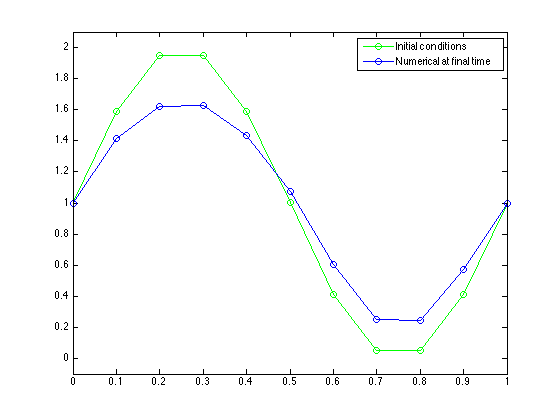
\includegraphics[scale=0.6]{before_numerical.png}
    \caption{Numerical Approach}
    \begin{minipage}{0.75\textwidth}
    {\footnotesize m = 11, dt = 0.005 for nt = 1, Numerical Approach}
    \end{minipage}
    \end{figure}
    
\begin{figure}
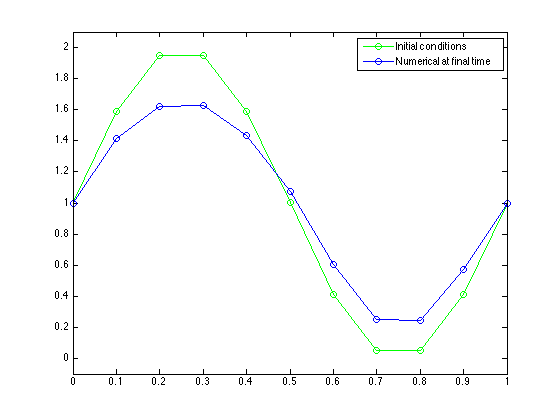
\includegraphics[scale=0.6]{after_analytical.png}
    \caption{Analytical Approach}
    \begin{minipage}{0.75\textwidth}
    {\footnotesize m = 11, dt = 0.005 for nt = 1, Analytical Approach}
    \end{minipage}
    \end{figure}
\end{center}  
\FloatBarrier
As we can easily figure out, the answers are identical to each other.

\item
The modification's time complexity is comparable to the triangular version's time complexity. Although we did N times iteration, rather than 3. But each iteration is simply to use the calculated formulas rather than evaluation F. So this modification has mineral changes to the overall time complexity.

\item Time Consuming\\

The test condition is at dt = 0.005 and nt = 10 :
    \begin{center}
    \begin{tabular}{c c}
    $ m = 161$ & $ t = 0.3412s$\\
    $ m = 321$ & $ t = 0.6129s$\\
    \end{tabular}
    \end{center}
    
\item
After comparison, we can find out that the triangular numerical approach and the analytical approach have the similar performance. But I think the numerical approach is more generic and the implementation is much more simpler. In term of result precision, I think there is no much difference, the numerical approach's result is acceptable. 
\end{enumerate}



    
    \section{Question 2}
    \subsection{Question a}
    By implementing the following formulas, we will get desired result which is the so called $F_{ijk} = 0$
    
    \begin{itemize}
    
    \item
    \begin{equation}
    \label{eq:x_dim}
    \frac{\partial}{\partial y}\left( c(u)\frac{\partial u}{\partial x}\right ) = \frac{c(u_{i+\frac{1}{2}})(u_{i+1}-u_i)-c(u_{i-\frac{1}{2}})(u_i-u_{i-1})}{\Delta x^2}
    \end{equation}
    
    \item
    \begin{equation}
    \label{eq:y_dim}
    \frac{\partial}{\partial y}\left( c(u)\frac{\partial u}{\partial y}\right ) = \frac{c(u_{j+\frac{1}{2}})(u_{j+1}-u_j)-c(u_{j-\frac{1}{2}})(u_j-u_{j-1})}{\Delta y^2}
    \end{equation}
    
    \item 
    \begin{equation}
    \label{eq:z_dim}
    \frac{\partial}{\partial z}\left( c(u)\frac{\partial u}{\partial z}\right ) = \frac{c(u_{k+\frac{1}{2}})(u_{k+1}-u_k)-c(u_{k-\frac{1}{2}})(u_k-u_{k-1})}{\Delta z^2}
    \end{equation}

    \end{itemize}
    
    Where $c(u)=1+u^2$. And we use compact space approximation to approximate $c(u)$ which is:
    \begin{equation}
    \label{eq:u+1/2}
    c(u_{i+\frac{1}{2}})=c\left(\frac{u_i+u_{i+1}}{2}\right)
    \end{equation}
    and:
    \begin{equation}
    \label{eq:u-1/2}
    c(u_{i-\frac{1}{2}})=c\left(\frac{u_i+u_{i-1}}{2}\right)
    \end{equation}
    individually.
    
    
    \subsection{Question b}
    
    Below are the running details, the data are from the program itself:
    \begin{center}
    \begin{tabular}{c c c c}
    Grid Dimension & System Size $N$& Iterations Number & Total Time $T$\\
    5 & 27 & 4 & $0.036451s$\\
    8 & 216 & 6 & $3.520961s$\\
    11 & 729 & 6 & $89.399273s$
    \end{tabular}
    \end{center}
    As we can see:
    \begin{center}
    \begin{tabular}{c c}
    System Size $N$& Time per Iteration $T$\\
    27& $ 0.0090s$\\
    216& $0.4401s$\\
    729 &$8.1273s$
    \end{tabular}
    \end{center}
    \FloatBarrier
    Which can be drawn as: 
    \begin{figure}
    \centering
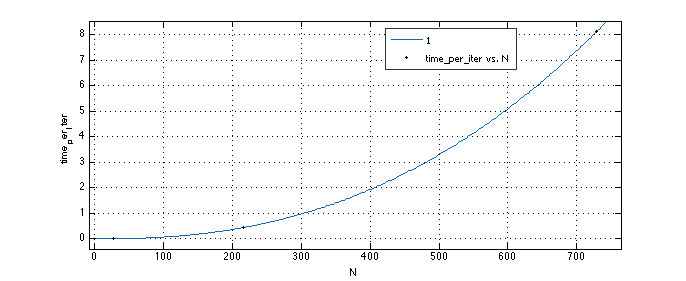
\includegraphics[scale=0.6]{Time_complexity.png}
    \caption{Simple Curve fitting}
    \begin{minipage}{0.75\textwidth}
    {\footnotesize $$f(x) = 1.117*10^{-06}x^{2.397}$$}
    \end{minipage}
    \end{figure}
    \FloatBarrier
So, The time complexity should be around $\mathcal{O}(n^2)$, which is :
$$T = \mathcal{O}(N^2)$$

\subsection{Question c}
The modified codes:

\begin{verbatim}
matlabLinearSolve.m

function x = matlabLinearSolve( A, b )

% function x = linearSolve( A, b )
%  Linear solution algorithm for the
%  system Ax=b 
% Input: nxn matrix A
%        n-dim column vector b
% Output: n-dim column vector x

% solve the system here

x = A\b;

end
\end{verbatim}
I verified that changing solver to use the "\textbackslash" operator will not change the computed result, and below is a example at dim=5:
\begin{verbatim}
>> temp = m_dim_5-dim_5

temp(:,:,1) =

     0     0     0     0     0
     0     0     0     0     0
     0     0     0     0     0
     0     0     0     0     0
     0     0     0     0     0


temp(:,:,2) =

     0     0     0     0     0
     0     0     0     0     0
     0     0     0     0     0
     0     0     0     0     0
     0     0     0     0     0


temp(:,:,3) =

     0     0     0     0     0
     0     0     0     0     0
     0     0     0     0     0
     0     0     0     0     0
     0     0     0     0     0


temp(:,:,4) =

     0     0     0     0     0
     0     0     0     0     0
     0     0     0     0     0
     0     0     0     0     0
     0     0     0     0     0


temp(:,:,5) =

     0     0     0     0     0
     0     0     0     0     0
     0     0     0     0     0
     0     0     0     0     0
     0     0     0     0     0
\end{verbatim}

\subsection{Question d}
\begin{itemize}
\item sparsePattern3DFD.m\\

Build the Jacobian matrix for PDE 3D model, and where there is a number an 1 will stands in that position. The output is in sparse format. It is column based, and organized in the increasing row order.

\item sparseJac.m\\

According to the given sparse Jacobian matrix from the function called \textit{sparsePattern3DFD.m}. This function uses greedy approach to give a function call strategy to eliminate the unnecessary function call while evaluating the Jacobian matrix.

\item buildJacobian.m\\

According to the given strategy from the function called \textit{sparseJac.m}, as well as the sparse Jacobian matrix model from the function called \textit{sparsePattern3DFD.m}. This function evaluate the Jacobian matrix and fill in the model from \textit{sparsePattern3DFD.m}.

\end{itemize}


\begin{center}
\begin{tabular}{c c}
Model Size & Function Calls Required \\
$m =5$&8\\
$m = 8$&10\\
$m = 11$&12
\end{tabular}
\end{center}
As we can from the above table, that because the Jacobian matrix is a pretty sparse matrix, using the greedy approach will fill in the blank left before. And thus the number of function calls increases slowly along with the increasing of the nonlinear system size N as well as the the size of Jacobian matrix itself.

However, if we use the standard numerical approach to calculate the Jacobian matrix, we need the following numbers function calls to finish each Jacobian matrix evaluation:

\begin{center}
\begin{tabular}{c c}
Model Size & Function Calls Required \\
$m = 5$& 8 $\rightarrow$ 27\\
$m = 8$&10 $\rightarrow$ 216\\
$m = 11$&12 $\rightarrow$ 729
\end{tabular}
\end{center}

Clearly, by improving the approach in solving the linear system, we have greatly increased the efficiency of the solver.

\subsection{Question e}

\begin{center}
\begin{tabular}{c c c}
Model Size & System Size & Time per iteration\\
$m = 11$ & $ N = 729 $ & $t = 0.0789s$\\
$m = 16$ & $ N = 2744 $ & $t = 0.2812s$\\
$m = 21$ & $ N = 6859 $ & $t = 0.7129s$
\end{tabular}
\end{center}

\FloatBarrier 
Which is:
\begin{figure}
\centering
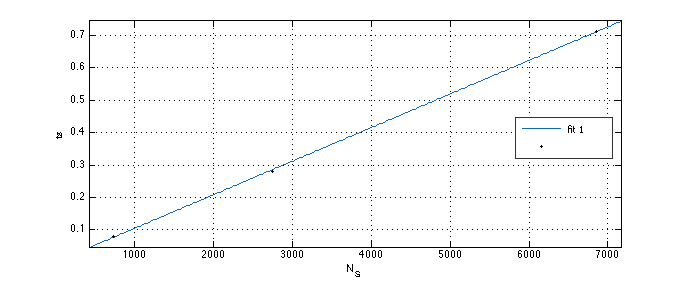
\includegraphics[scale=0.6]{curve_fit2.png}
    \caption{Simple Curve fitting}
    \begin{minipage}{0.75\textwidth}
    {\footnotesize $$f(x) = 0.0001*x+0.0007$$}
    \end{minipage}
    \end{figure}
    \FloatBarrier
So, The time complexity should be around $\mathcal{O}(n)$, which is :
$$T = \mathcal{O}(N)$$
\FloatBarrier

\subsection{Question f}

\begin{enumerate}
\item The problem itself:
\begin{itemize}
\item runFDM.m

Function call controller.
\item rhs.m

Right hand side of the PDE problem.

\item fdm3D.m

The nonlinear system itself.

\end{itemize}


\item 3D finiate difference model:

\begin{itemize}
\item sparseJac.m

This one is for the 3d sparse system, it calculates the function call strategy.
\item sparsePattern3DFD.m:

This one is suitable to all the 3d sparse linear system. It generates a sparse Jacobian matrix.
\item newtonAlgorithm.m

A basic Newton method.

\item lineSearch.m

Update method for Newton method.

\item index3DMesh.m

Calculate mesh for the 3D index.

\item index3DFD.m

Calculate vector index for the 3D system.

\item fdJacobian.m

Calculate the Jacobian matrix.

\item buildJacobian.m

Calculate the Jacobian matrix. Optimized for the sparse system. 
\end{itemize}



\item sparse nonlinear system :

\begin{itemize}
\item vectorTOmesh.m:

This one is simply a vector manipulation 
\item matlabLinearSolve.m

Linear system solver using matlab's $\backslash$

\item linearSolve.m

Linear system solver.


\end{itemize}

\end{enumerate}





\end{document}
